\newpage
\section{Technology and Market Impact on Operating Systems}
\subsection{Problem:}
Some years back, operating systems played a critical rule in changing worldwide technologies and the
market, and consequently drove what trended at that time. While this may be true as well today, it is also
true that technology trends are also changing and impacting operating systems in many different ways. In
this question, you will need to use the concepts learned in class to go beyond what was covered. In other
words, you will need to use what you have learned and understood in class to conduct a small research,
which surely include ideas, subjects, technologies, market pressures, etc., which were not explicitly
covered in class. In particular, your research needs to look/examine the last 5 years or so, as well as the
next 5 years as you can anticipate from available predictions on the subjects.

\newpage
\subsection{Technology trends in the past 5 years}
For each of the following subjects/matters, describe how technology trends in the past 5 years
impacted this subject, in relation to operating systems, (or impacted operating systems in
relation to it!). You should be as comprehensive as possible (comment on different relevant
aspects, such as performance, cost, ……etc.)

\subsubsection{IoT (Internet of Things)}

IoT plays a vital part in the development of OS in general. In the past five years, it has been growing significantly, becomes a boot for new innovations in Operating Systems field. 
There are a great number of IoT OSs that were developed in order to fit this new recent trend such as Contiki-OS, RIOT and Zephyr. They are most well -known for compatibility with hardware restrictions and battery limitation. 
Consequently, it tackles successfully the resource-constrained problems of IoT gadgets.  \\
In the past, it was a challenge to develop a stable connection to the Internet from an IoT device due to its limitation in term of Hardware. However, most IoT OSs has been developed to have complete networking compatibility despite of its nature constraints (Zikria et al., 2019). Moreover, most of IoT OSs also has supported multi threading, providing a faster compute speed than any Uni-programming supports before. \\
The overview of common IoT OSs and its abilities is on the table following [1]

\begin{centering}
    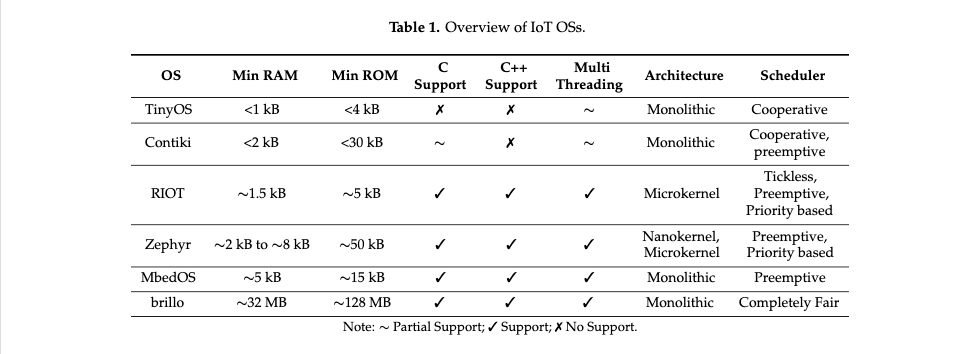
\includegraphics[scale=0.5]{IoTOS} 
\end{centering}

Even though the growth of IoT and IoT OSs is considerable, it still exists several issues that need to be address. The problems that engineers are facing can namely be energy efficiency for IoT devices and network connectivity since they are not advanced enough to achieve certain tasks. However, the arises of IoTs not only has greatly inspired the OS field, it also opens a new horizon for OS developers to work on more efficiency systems and overcome the limitations.

\subsubsection{CPU processing (speed, capacity, cores, etc.)}

There is a dramatical changes in CPU processing in recent years. The CPU is now capable of working with Augmented Reality (AR).
Thus, it has an impact to the OS to provide the needed API to integrate with the applications. 
This advancement means the traditional OS with multi threading model need to be improved.
In another aspects, there are a number of research on multi core programming to expand the potential of all the cores in CPU nowadays.
Multi core programming is the solution for concurrent systems for multi processor systems, and it is being researched carefully across the globe.
The field is receiving attention from engineers and computer scientists since it is believed to not only greatly reduce the price point of CPU, but also reduce the dependent on hardware by optimizing the CPU with softwares. \\
However, the field is currently under developing.

\subsubsection{Main Memory (i.e. RAM)}
Despite the rapid changes in other fields, memory technology is staying essentially the same at its core in the past few years. 
Although it is noticeable that the main memory now is compact and smaller than ever before with the capacity growing each year, the mechanism to control and manage RAM is still the same. 
In another word, computer organization remains the same through out the years.\\
\\
In the other hand, RAM reliability has been greatly improved. The error management now can handle the failure mechanism called \textit{row hammer} in the past. 
Also, in the past five years, manufacturers have made the price of main memory more accessible to the general public. For example, the price of 8GB RAM in the past 5 years is much higher than nowadays, even with inflation adjusted. \\
\\
In conclusion, memory technology unlike other technology, has grown stably. It achieved success in extending the limitation of memory compact with a reduced cost, but the integration with Operating Systems seen a little changes.

\subsubsection{Cloud Computing}
In the new decade, many companies and enterprise are changing to cloud computing to reduce the cost for infrastructure, and allow flexibility of the server. This trend effects considerably on how Operating systems is being developing. 
In the past few years, Internet has been more and more accessible for people all over the world; thus, increases demand for hosting website and management. Internet usage saw a significant increase in recent years. 
Being inspired by that trend, operating systems are experiencing a rapid development for multiple users instead of the traditional model of one single user, one single system.
Nowadays, an user can easily connect to a host and get access to data to process his/her job via the Internet. Cloud computing opens a new perspective for the society as it does not depend solely on the hardware requirements as before.
It offers users with great convenience and ease of out dated hardware.
With that changes, the OS for cloud computing services have to be developed to accommodate the growing demands. 
In the past years, the OS to manage the infrastructure of cloud hosting services were dramatically improved to offer more secure, and more accessible to users.\\
\\
On another aspect, there are some critical issues with Web based OS that companies are facing. Since the database of a business is located in the server of a third party, there is a rising concern about security problems. That requires the OS to evolve and secure its access. 
Moreover, the OS on the cloud has to be stable since there are many users depend on it for daily basic works. \\
\\
In conclusion, cloud computing offers a turning point for the development of OS. It shifts the traditional OS to a new aspect of modern work. 
Despites its existing disadvantages, it is still an evolution of operating systems.

\newpage
\subsubsection{Big-data Processing}
In recent years, data is proving its important for business. Especially for large enterprises such as Google, Amazon, Facebook,.. Big data is essential to how they gain profits. Therefore, its impact on how operating systems are designed is undoubtedly. 
For large companies, the OS for their data server must be secured and fast enough for analytics. 
With these criteria, it can be observed that OS there is a need for OS to develop. 
Data analytics is also relying on a fast and reliable OS to complete business's work. There were new innovations such as Apache Spark for managing Data Source interface. It provides an easier tool for analyst to achieve the data they need. 


\newpage
\subsection{Technology trends anticipate in the next 5 years}
For each of the following subjects/matters, describe how “you anticipate” that very recent
and future technology trends in the short-term of the next 5 years will impact this subject, in
relation to operating systems (or impact operating systems in relation to it). You should be as
comprehensive as possible. Remember that your answer should reflect your own anticipation
based on your research

\subsubsection{5G Networks}

Nowadays, there is a currently a 5G war between nations in the world. 
5G is the fifth generation of wireless communications technologies that is promised to provide the connectivity that was ever available before. 
With the new technology, the limitation Internet speed might no longer exist in the upcoming years. As a result, cloud computing could be stronger than ever.\\
\\
On the business side, it will be a challenge that companies have to drive resources into developing Web based OS that is capable to accommodate such huge amounts of requests while securing the database. 
On the customer aspect, we can expect a shift from traditional OS to Web OS and the rise of Web Applications since it is already very popular and the average Internet usage of people will increase as 5G is starting.
More technologies for WebOS could be developed; thus, allowing developers more flexible on either learning or maintain the system. 
Moreover, unlike the traditional OS, WebOS would allow software providers to maintain and keep track of its user experience much easier. Hence, user's satisfaction can be increased. \\
\\
In conclusion, 5G technology offers a faster speed to connect to the web. Thus, it empowers the development for new OS innovations.

\subsubsection{Artificial intelligence}

Artificial intelligence (A.I) is the future undoubtedly as more and more businesses are using for a variety purposes such as predict customer behaviours. 
It is being applied to many fields nowadays as it opens a new aspect of computing and research. \\
\\
First of all, to train an AI model, the need for computing a large set of data is inevitable.
However, personal hardware or computers might not have enough computing speed to execute such a heavy task.
Therefore, cloud computing in a remote server is a must for developers working with AI.
Operating systems have to evolve to have enough computation power to serve the requests for training AI model. \\
\\
Furthermore, AI training depends hugely on the data set it is provided. 
As a result, data set has to be analyzed and sorted in purpose to create an accurate model and produce the correct outcomes.  
This demands a system of big data efficient enough for big enterprises which rises a demand to implement an OS structure that is reliable and fast enough. 
Therefore, we could expect a huge development in server OS and system manager in the next few years.
\\
\\
In conclusion, artificial intelligence is a technology that is expanding with an unstoppable speed.
It is also rising new OS needs in the future and new technologies might be invented to board these needs.


\subsubsection{Main Memory (i.e. RAM)}

Memory technology is expected to grow stably in the next 5 years. But it will affect the future of OS development. \\
\\
Firstly, the memory-centric architectures are gaining attention from researchers. This is because the advancement of processor is expected to reach its peak soon. 
Moreover, data is becoming the new currency; thus, memory is more valuable than ever before. 
As this is a rising trend, OS will probably be focused on utilizing the pool of memory and expand its ability for faster memory access. 
In addition, memory error handling in OS will be improved over time as the risk of losing valuable memory is more dangerous than before.
The OS will be evolved such that memory errors at big scale can be minimized. \\
\\
To be concluded, the next five years might be the years that the world shifts attention to memory-centric OS, and manufacturers start to improve memory technology.


\subsubsection{Reacting to world pandemics, such as the current COVID-19 }

In the next five years, the technologies might have been developed enough for the world to cope with another pandemic such as COVID-19 once again. \\
\\
With the active development of Web OS, and 5G networks, it will be eased for employers to switch workplace from traditional office to home office.
The transition might get smoother as people are having better tools.
In addition, people will be less depend on hardware systems at home. 
Since employers can connect to workplace and do usual works regardless of the specs on their home computer, the work flows in an office might remain the same. \\
\\
Furthermore, with better technologies in terms of connectivity, hosting, computing speed, we can be benefited with more reliable data. 
With accurate data, nation leaders will have a broader vision on how spread a pandemic are; thus, actions and measures will be taken at the right time, helping to prevent the spread. \\
\\
With the rate of new development in technologies, it can be predicted that citizens of the world will have a better preparation in the next pandemic.

\subsubsection{Fault-tolerance}

In the future, it is expected that fault will have less impacts than before. \\
\\
There might be more advanced failure handling to be embedded in the OS to response to the failure.
For example, the system might be backed up frequently; therefore, in case of failure, the system can easily shut down and recover the data with the processes it is executing.
With a large scale infrastructure, the OS might be implemented so that it triggers a backup system to cope with failure immediately.
Thus, in the event of system downs, user experience might not be interrupted. 
To achieve this goal, the OS in the server has to have a special fast response mechanism for failure.
The implementation of such system will be very expensive at the moment. 
However, with the rapid development of OS, the cost is predicted to be lowed in the future
\\
In conclusion, with the rising of needs for such improvement, most large and medium infrastructure might be able to afford a system for fault tolerance that is fast enough to not interrupt user experience in the system.

